\section{Correlated Multi-Armed Bandit Model}
\seclabel{background}

Finding an approximate solution of Equation~\ref{eq:objective} with Multi-Armed Bandits requires a predictive model of the probability of force closure for each grasp.
We use Continuous Correlated Beta Processes (CCBPs) to model force closure for a grasp as a Bernoulli random variable with correlations across grasps and objects~\cite{goetschalckx2011continuous, montesano2012active}.
\figref{correlated-motivation} illustrates how using a correlated model can lead to accelerated convergence of bandit algorithms.
%In practice, correlations may occur between two grasps that contact the same shape in similar locations, or between grasps on different shapes, such as grasping the handle of a mug and the handle of a teapot.

\begin{figure}[t!]
\centering
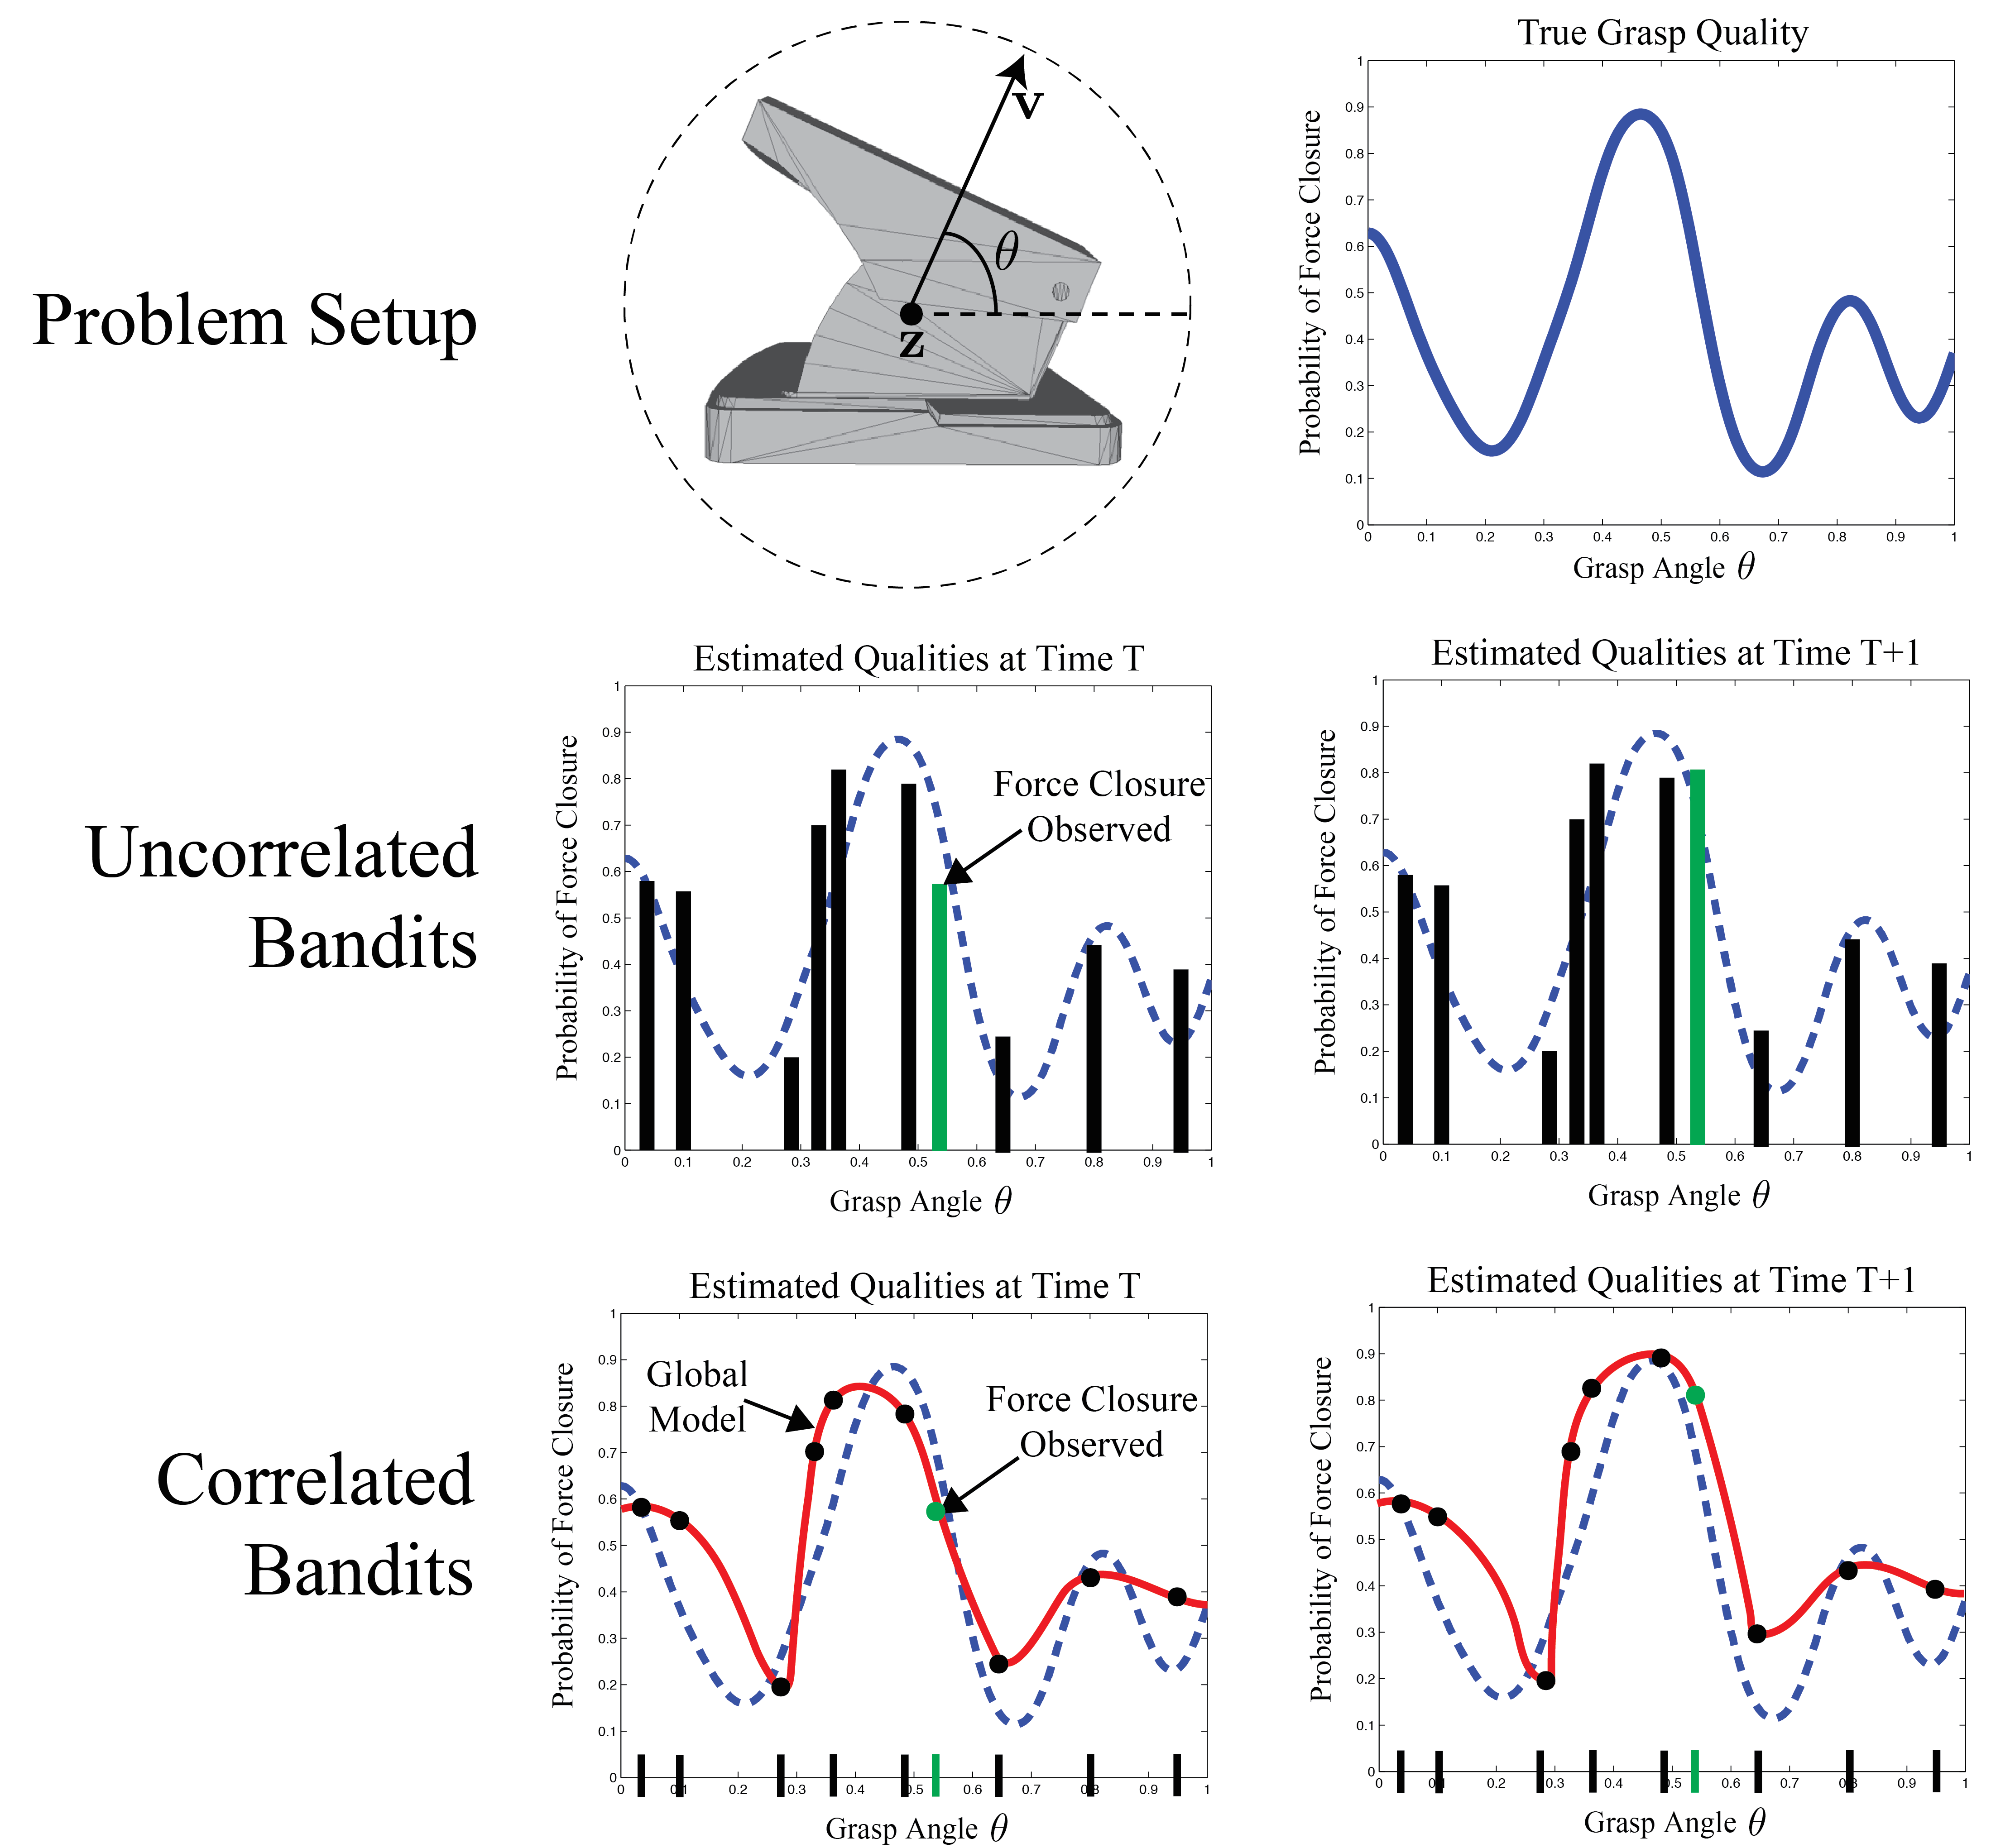
\includegraphics[scale=0.23]{figures/illustrations/correlated_bandits.png}
\caption{(Top Left) Consider a set of grasps with fixed center at an object center of mass and approach direction sampled along a one-dimensional circle. (Top Right) The true probability of force closure $P_F$ as a function of the angle of the grasp axis. (Middle Left) Uncorrelated MAB models maintain an estimate of $P_F$ independently for each grasp, indicated by bars and their height. On iteration $T$ of a MAB algorithm, the evaluated grasp (green bar) is force closure for samples . (Middle Right) Only the estimate of $P_F$ for the sampled grasp is updated on iteration $T+1$, and the grasp with highest estimated $P_F$ remains suboptimal. (Bottom Left) Correlated MAB models maintain a global predictive function (red) of $P_F$ for any possible grasp but may select grasps from a set of discrete candidates (indicated by dots). (Bottom Right) On iteration $T+1$, the evaluated grasp (green dot) is sampl returns force closure and the global model is updated, increasing the estimated $P_F$ for ``nearby" grasps. Although a suboptimal grasp was sampled, the global model now correctly predicts the optimal grasp in the set. }
\figlabel{correlated-motivation}
\vspace*{-15pt}
\end{figure}

\subsection{Continuous Correlated Beta Processes}

Continuous Correlated Beta Processes (CCBPs) were independently proposed by Goetschalckx et al.~\cite{goetschalckx2011continuous} and Montesano and Lopes~\cite{montesano2012active} to model correlations between the Bernoulli random variables in a Beta-Bernoulli process, which may lead to faster convergence in MAB problems~\cite{chu2011contextual}.
Such correlations may exist when the Bernoulli random variables depend on common latent factors.
For example, two grasps may have similar $P_F$ when they contact the same shape in similar locations or the surface geometry at the contact points is similar, such as a grasp on the handle of a mug and the handle of a teapot.

We are interested in solving Equation~\ref{eq:objective} for a new object $\mO_i$.
Let $\mG_{i}$ be a set of $K$ candidate grasps for $\mO_i$, $\Gamma_i = \{\bg_{i,k}\}_{k=1}^K$.
We define $F_{j,\ell} = F(\bg_{j,\ell}) \in \{0, 1\}$ an occurence of force closure on an evaluation of any grasp $\bg_{j,\ell}$ on object $\mO_j$ using samples of object pose, gripper pose, and friction, as described in \secref{quality}.
Then let $N_{j,\ell}$ be the number of total evaluations of for grasp $\bg_{j,\ell}$, and define $S_{j,\ell} = \sum_{a=1}^{N_{j,\ell}} F_{j,\ell}$ to be the total number of times force closure has been observed for any grasp.
Futhermore let $\mD = \{ N_{j,\ell}, S_{j,\ell}, \mY_{j,\ell} = (\bg_{j,\ell}, \mO_j) \big| j = \{1, ..., M\}, \ell \in \{1, ..., K\} \}$ be a discrete set of $M$ known objects stored in a database, each with a discrete set of $K$ candidate grasps $\Gamma_j = \{\bg_{j,\ell}\}_{\ell=1}^K$ and $N_{j,\ell}$ and $S_{j,\ell}$ for each object.

%and let $\mS = \{ S_{j,\ell} \big| j \in \{1, .., M\}, \ell \in \{1, ..., K\} \}$ be the history of force closure observations for all grasps and all objects in the database.

We model force closure for each candidate grasp, $F_{i,k}$, as a Bernoulli random variable with probability of success $\theta_{i,k}= P_F(\bg_{i,k})$.
Since we do not know the value of $\theta_{i,k}$, we maintain a belief distribution for each $\theta_{i,k}$ based on our prior belief about the likelihood of force closure.
In CCBPs, the belief distribution on the Bernoulli parameter $\theta_{i,k}$ is the Beta distribution, which is specified by shape parameters $\alpha > 0$ and $\beta > 0$:

\vspace{-2ex}
\begin{align*}
	\betadist(\alpha, \beta) = \frac{1}{B(\alpha, \beta)} \theta_k^{\alpha-1} (1 - \theta_k)^{\beta-1}
\end{align*}

A CCBP estimates the shape parameters for a grasp and object $\mY_{i,k} = (\bg_{i,k}, \mO_{i}) \in \mM$ using a normalized kernel function $k(\mY_p, \mY_q) : \mM \times \mM \rightarrow [0,1]$ that measures similarity between a pair of grasps and objects from the Grasp Moduli Space $\mM$.
The kernel approaches 1 as the arguments become increasingly similar and approaches 0 as the arguments become dissimilar.
In this work we use a unit-bandwidth squared exponential kernel 
\begin{align*}
	k(\mY_p, \mY_q) &= \exp\left( - \frac{1}{2} \sum \limits_{m=1}^{N_f} \|\phi_m(\mY_p) - \phi_m(\mY_q)\|_{W_m}^2 \right)
\end{align*}
\noindent where $\phi_m: \mM \rightarrow \mathbb{R}^{d_m}$ for $m = 1, ..., N_f$ are feature mappings for a grasp and object to a $d_m$-dimensional Euclidean space, $W_m \in \mathbb{R}^{d_m \times d_m}$ are linear transformations scaling the relative contribution of the feature maps to the similarity metric, and $\| \phi \|_{W} = \phi^T W^T W \phi$.

Before the first iteration of the MAB algorithm, we update our belief for each candidate grasp to its similarity to all grasps and objects from the database $\mD$ as measured by the kernel~\cite{goetschalckx2011continuous}:
%\vspace{-2ex}
\begin{align}
	%p \left(\theta_{i,k} | \mS, \mN \right) &= \betadist\left( \alpha_{i,k,0}, \beta_{j,k,0} \right) \notag \\
	\alpha_{i,k,0} = \alpha_{0} & + \sum \limits_{j=1}^M \sum \limits_{\ell=1}^K k(\mY_{i,k}, \mY_{j,\ell}) S_{j,\ell} \label{eq:alpha-prior} \\
	\beta_{i,k,0} = \beta_{0} & + \sum \limits_{j=1}^M \sum \limits_{\ell=1}^K  k(\mY_{i,k} \mY_{j,\ell}) (N_{j,\ell} - S_{j,\ell}) \label{eq:beta-prior}
\end{align}
\noindent where $\alpha_{0}$ and $\beta_{0}$ are prior parameters for the Beta distribution~\cite{laskey2015bandits}.
% and $\mS$ and $\mN$ are the number of successes and total trials for grasps in the database, respectively.
Upon observing $F_{i,k}$ for grasp $\bg_{i,k}$ on iteration $t$, we update our belief $\theta_{i, \ell}$ for all other grasps on object $\mO_i$ by~\cite{goetschalckx2011continuous}:

\vspace{-2ex}
\begin{align}
	\alpha_{i,\ell,t} &= \alpha_{j,\ell,t-1} + k(\mY_{i, \ell}, \mY_{i,k}) F_{i,k} \label{eq:alpha} \\
	\beta_{i,\ell,t} &= \beta_{j,\ell,t-1} + k(\mY_{i,\ell}, \mY_{i,k}) (1 - F_{i,k})\label{eq:beta}
\end{align}

\noindent Intuitively, this allows observations of one grasp to constitute fractional observations of similar grasps.

\subsection{Feature Mappings}
We use a set of feature mappings $\phi_1, ..., \phi_{N_f}$ to capture similarity based on grasp parameters, local surface geometry, and global object shape.

\subsubsection{Grasp Parameters}
\seclabel{param-features}
Since grasps may be correlated across small changes to the grasp center and approach direction on a single shape, we use the feature maps $\phi_{x}(\mY) = \bx$ and $\phi_{v}(\mY) = \bv$, the identity transformations for the grasp center and axis.
Additionally we use the moment arm feature map $\phi_{\rho}(\mY) = [ \| \rho_1 \|_2, \| \rho_2 \|_2]^T \in \bR^2$ because points on the object surface with larger moment arms will move greater distances under object orientation uncertainty.
However, similarity between grasp centers and approach directions may not indicate similar $P_F$ if the surfaces near the contact locations are dissimilar.
For example, consider two grasps that contact a box near the corner.
The two grasps may have similar parameters and moment arms but may contact the surface on different sides of the edge, resulting in different surface orientations at the contact points.

\subsubsection{Grasp Heightmaps}
\secref{local}
We also use a variant of the grasp heightmap features of Herzog et al.~\cite{herzog2012template} and Kappler et al.~\cite{kappler2015leveraging}.
Let $d_h \in \mathbb{Z}$ be the number of pixels along each dimension of the heightmap, let $\mP = \{-d_h, ..., d_h\}$ be the row / column pixel indices for the heightmap, let $\delta \in \mathbb{R}$ be the resolution of the image pixels in meters, and let $r \in \mathbb{R}$ be a minimum projection distance.
Furthermore, let $\bc_i, i = 1, 2$ be a contact point for grasp $\bg$ and let $\bt_1, \bt_2$ be two orthogonal unit vectors to the grasp approach direction $\bv$.
Our heightmap at contact $i$, $\bh_{i}: \mP \times \mP \rightarrow \bR$, maps discrete locations along the tangent plane specified by $\bt_1, \bt_2$ to the distance to the surface along the grasp axis $\bv$.
To compute the heightmap value at pixel $u,v \in \mP$, we first compute the 3D location of the pixel on the plane $\bp_i(u,v) = \bc_i + \delta u \bt_1 + \delta v \bt_2$.
Then we assign the heightmap value
\begin{align*}
	\bh_k(u,v) = \minimum{t \geq -r} t \text{ such that } | f\left( \bp_k(u,v) + s_k \bv \right) | < \epsilon
\end{align*}
 where $s_1 = -1$, $s_2 = 1$, $\epsilon$ is the surface threshold used for finding contacts, and $f$ is the SDF of object $\mO$. 
Finally, we make the heightmap rotationally invariant by rotating it to align the axes with the eigenvectors of the weighted covariance matrix of contact points generating the heightmap as described in~\cite{tombariunique}.
Our full feature vector for the heightmaps is $\phi_{h}(\bg_i, \mO_i) = [\bh_1, \bh_2]^T$. \TODO{Describe symmetrization of heightmaps for contacts.}
\figref{local-feature-model} illustrates local surface patches extracted by this procedure.

\begin{figure}[t!]
\centering
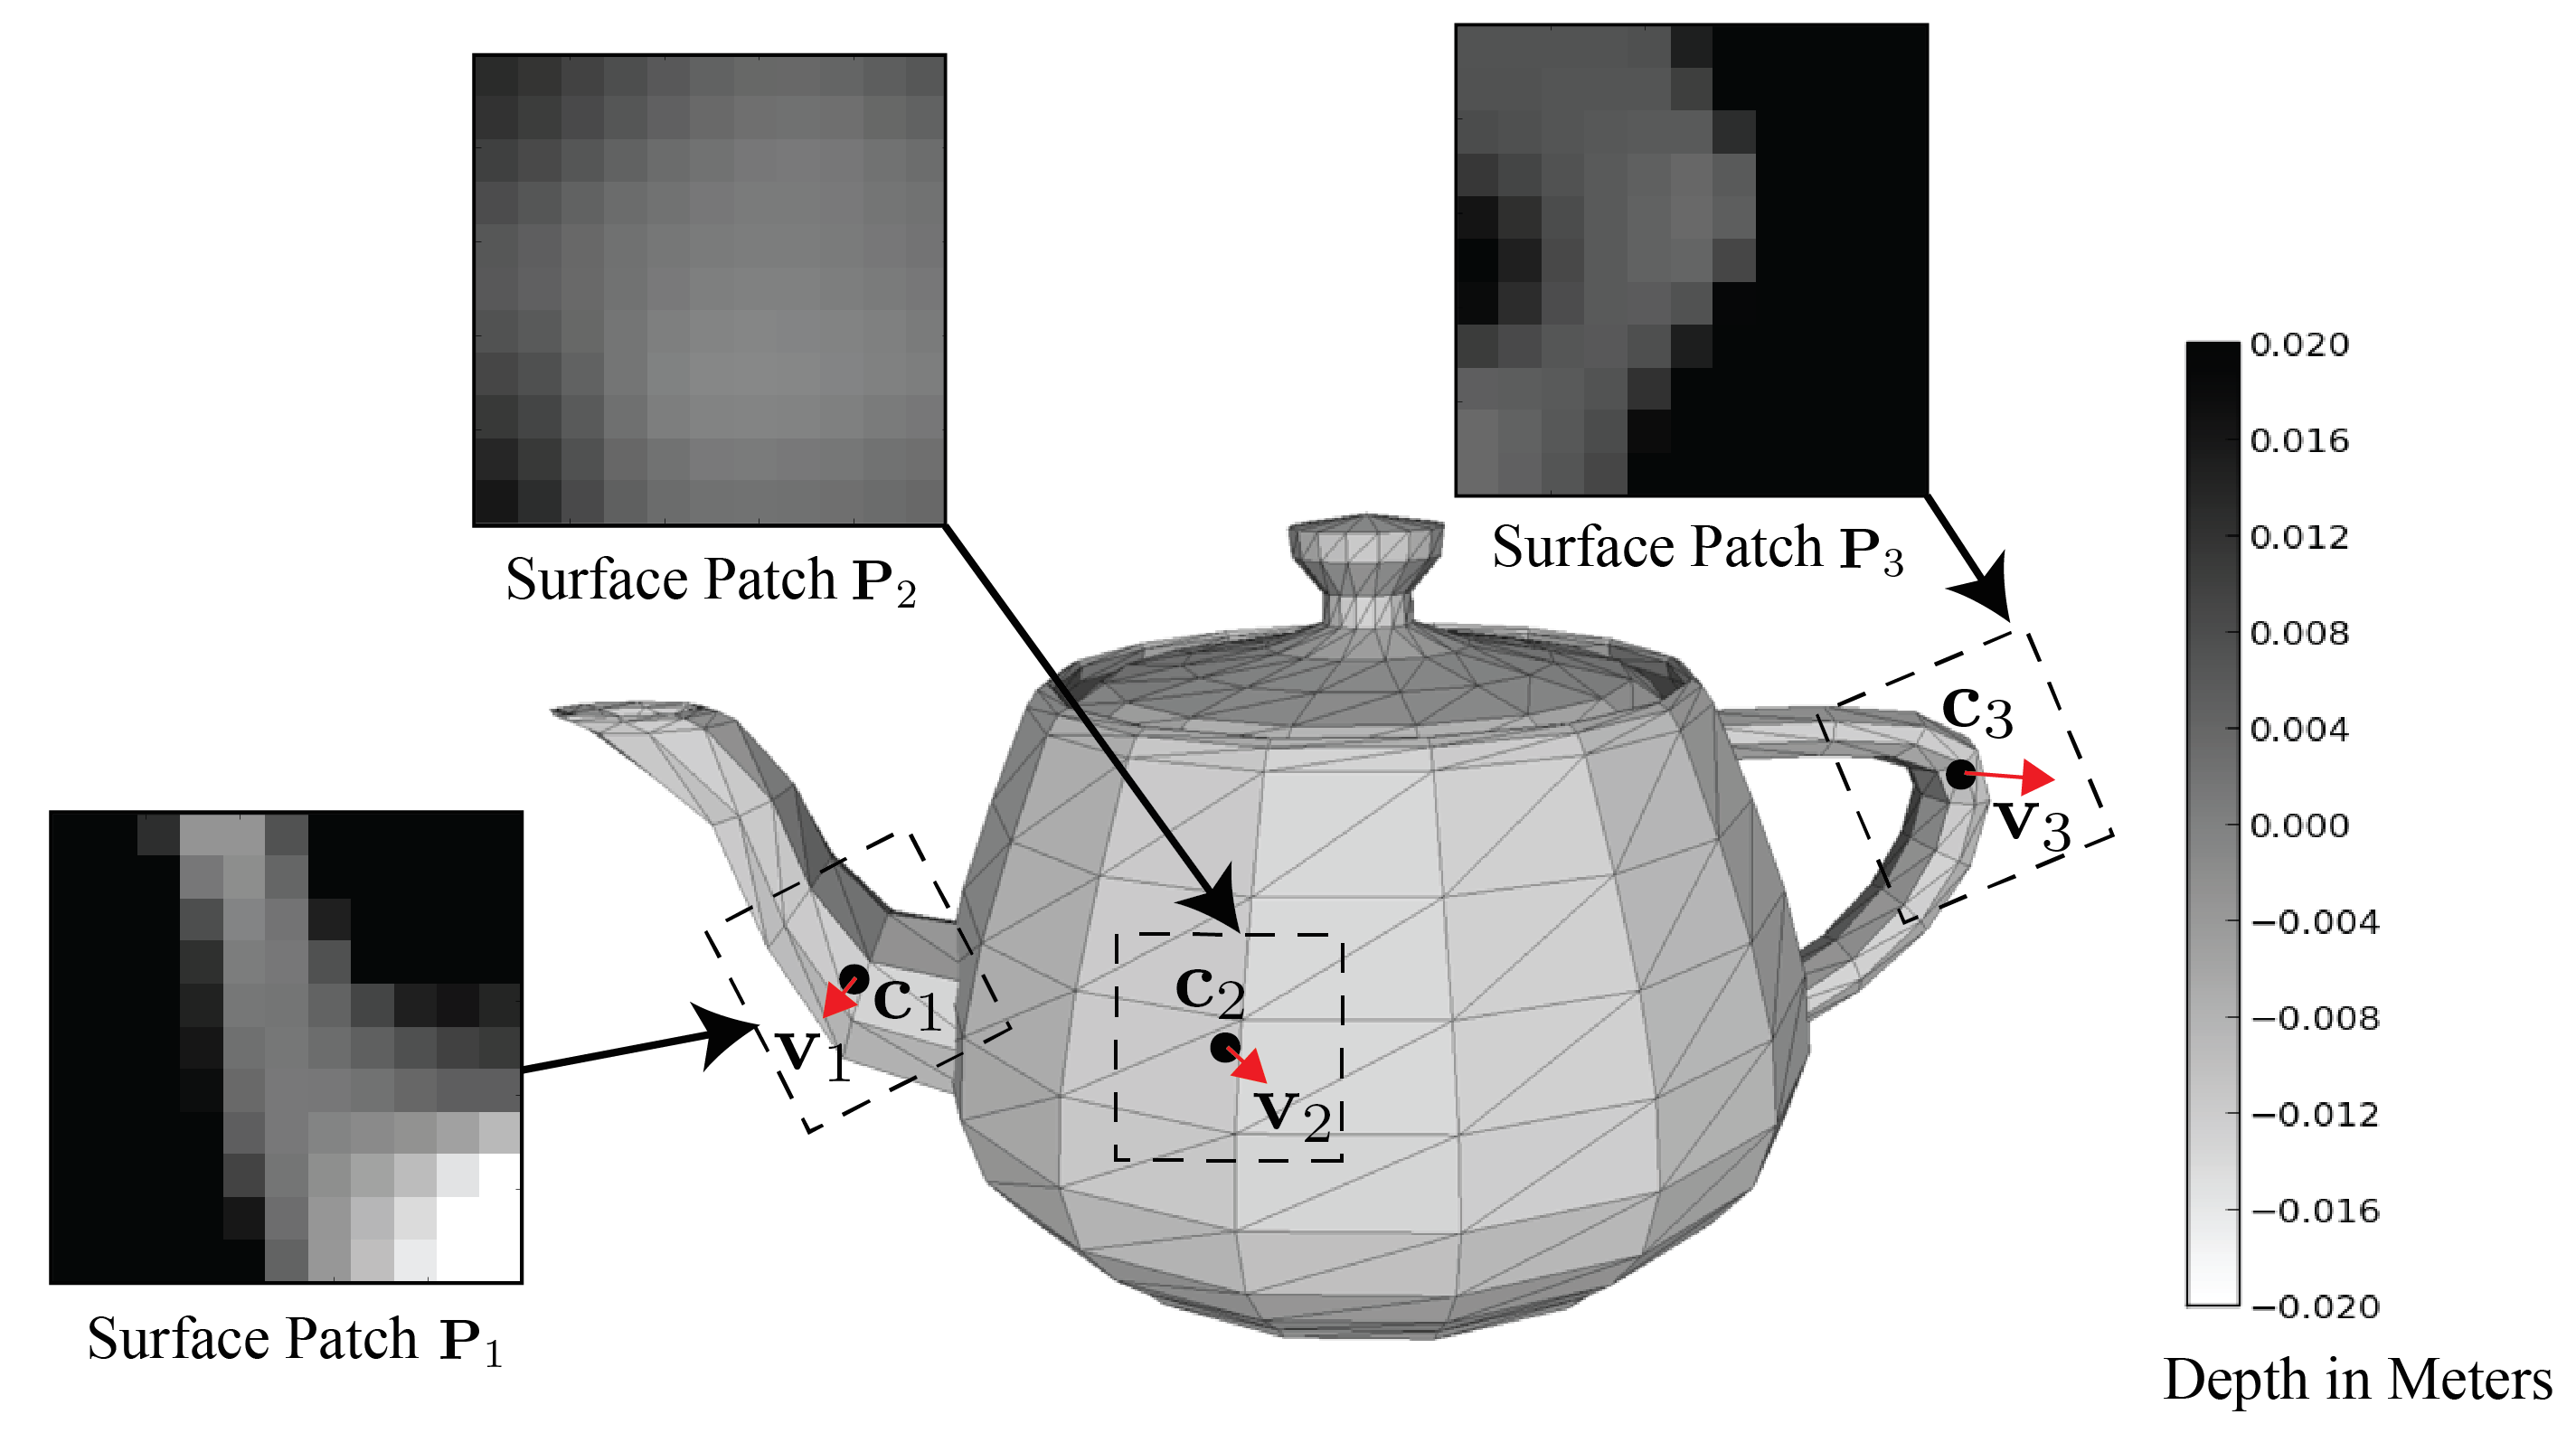
\includegraphics[scale=0.35]{figures/illustrations/local_feature_model.png}
\caption{Three local surface heightmaps extracted on a teapot. Each heightmap is ``rendered" along the grasp axis at each contact point and oriented by the local directions of maximum variation in the heightmap.  }
\figlabel{local-feature-model}
\vspace*{-15pt}
\end{figure}

\subsubsection{Global Features}
\seclabel{cnn}
While force closure is based on local surface properties of an object around contact points, measuring global similarity may be similarity may be useful for two reasons.
First, the sums in Equations~\ref{eq:alpha-prior} and~\ref{eq:beta-prior} may be expensive when the database is large, and global object similarity can be used to sum over only the objects that are grasped similarity to a new object of interest.
Second, the heightmaps may not capture all possible contact points for a grasp under perturbations in object and gripper pose.

%\TODO{Justify why class labels help, if they do}
We measure global similarity between objects using a feature mapping derived from multi-view Convolutional Neural Networks (CNNs)~\cite{su2015multi}, a state-of-the-art method for 3D shape retrieval.
\figref{global-feature-model} illustrates our method.
Let $R$ be the maximum dimension of the object bounding box.
We first render every object on a white background in a total of $N_c$ virtual camera views oriented toward the object center and discretized on a viewing sphere along angle increments $\delta_{\theta} = \frac{\pi}{N_c}$ and $\delta_{\phi} = \frac{\pi}{2 N_c}$ and radii $r = R, 2R$.
Then we train a deep CNN with the architecture of AlexNet~\cite{krizhevsky2012imagenet} to predict a class label for the rendered images based on known class labels for the 3D models using Stochastic Gradient Descent (SGD).
Next, we pass each of the $N_c$ views of each object through the finetuned CNN and max-pool the output of the fc7 layer.
We finally use Principal Component Analysis (PCA) to reduce the max-pooled output to from 400 dimensions to 100 dimensions.
This yields a representation $\psi(\mO) \in \mathbb{R}^{100}$ for each object, and thus our final feature map is $\phi_{g}(\mY) = \psi(\mO)$.
In our implementation, we trained the multi-view CNN on rendered images of 171 classes of 3D models from the SHREC 2014 dataset ~\cite{li2015comparison} for 500,000 iterations of SGD, which had a test accuracy of 76\%.

%\TODO{Expand above paragraph, include more details on method as well as the results of training}

\subsection{Optimizing Feature Weights}
One remaining issue is the selection of the relative feature weights $w_1, ..., w_{N_f}$.
We select the weights that minimize the cross entropy loss~\cite{de2005tutorial}:

\begin{align*}
	w_1^*, ..., w_{N_f}^* = \myargmin{w_1, ..., w_{N_f} \geq 0} \frac{1}{M} \sum \limits_{i=1}^M &\mu_i \log \left( \frac{\alpha_i}{\alpha_i + \beta_i} \right) + \\  &(1 - \mu_i) \log \left( \frac{\beta_i}{\alpha_i + \beta_i} \right)
\end{align*}
\noindent where $\alpha_i$ and $\beta_i$ are the posterior shape parameters given by Equations~\ref{eq:alpha-prior} and~\ref{eq:beta-prior} and $\mu_i$ is the probability of force closure evaluated by exhaustive Monte-Carlo integration for a set of $M$ grasps.
We optimize this objective using SGD with the weights initialized to $w_i = 100$ for all $i$.
\TODO{For experiments so far we actually use a grid search and not SGD but we are interested in using this in final experiments.}